\chapter{Research Proposal}

In this work, we propose the formulation of a preferential sampling scheme incorporating and formalizing some of the preliminary ideas proposal by Wellman \cite{wellmann2013information}. In particular, for practical applications, we propose a framework that integrates both preferential sampling schemes and the statistical information obtained from \emph{MPS} and training images. Our conjecture is that preferential sampling design by \emph{information theoretic} principles are distributed in facies transition zones and, consequently, can achieve enhanced reconstruction of channelized geological structures. We propose the use of maximum entropy based preferential sampling as a concrete alternative to classical sampling schemes.  

We present a new adaptive sequential empirical maximum entropy sampling (\emph{AdSEMES}) approach that integrates \emph{information theoretic} concepts for sampling design and prior information from training images. This scheme can be seen as a way of find the transitions zones of facies of interest. Thus, we formalize and implement three maximum entropy sampling schemes within the context of regionalized categorical variables with spatial dependence.


\section{Questions}

\begin{itemize}
	\item Given $K$ available measurements, what is the \emph{best} location for each one?
	\item Given an image model, is there a sampling regime where optimal sampling can outperforms classical approaches?
	\item How the previous gain is a descriptor of the complexity of the model?
	\item What is the best inference methodology for the proposed optimal sensing strategy?
	\item If the inference methodology correspond to \emph{MPS} approaches, can entropy and mutual information be good predictors of the performances?
\end{itemize}



\subsection{Main Objective}
\label{sec_Main_Obj}
% 5. Sate the general and specific objectives.

The main objective for this research proposal is the development of methods to assist the reconstruction of images describing \emph{2-D} binary regionalized variables by the use of \emph{sensing design} tools and the selection of appropriates inferences strategies. First, we take advantage of information theoretical tools for the formulation and implementation of adaptive sensing schemes. We focus on regionalized variables with several spatial dependence assumptions by taking advantage of spatial structure and other side knowledge of the media of interest. Second, given several sensing schemes, we evaluate \emph{ad-hoc} inference techniques addressing practical limitations related with the problem complexity. In addition, a comprehensive study of the integration of both adaptive sampling and inference methods is proposed under several preferential and no-preferential sensing schemes. 

\subsection{Specific Objectives}
\label{sec_Spec_Obj}

The specific objectives of this research proposal are:

\begin{itemize}
	\item Formalize a theoretical framework for optimal sampling design in \emph{2-D} regionalized variables. 
	\item Develop an adaptive sensing design framework using \emph{joint entropy} and \emph{mutual information} to measure uncertainty and spatial structure. 
	\item Compare performance of combinatorial, sequential and adaptive sampling design schemes.
	\item Study the stopping criteria for each sampling design in function of the capacity of an additional measure of improve the field characterization.
	\item Study a family of Markov random field models to describe spatial correlation on finite alphabet regionalized random variables.
	\item Study empirical statistic sources (\emph{MPS} and training images) to estimate the spatial dependence.
	\item Integrate the concepts of sensing design and inference methods on an adaptive sensing approach for the reconstruction of \emph{2-D} binary permeability channels.
\end{itemize}






\section{Hypotheses}

The main hypotheses for this proposal are the following:

\begin{itemize}
	\item At low acquisition regimes, the incorporation of prior information in the design of sampling schemes improves the performance of classical geosciences approaches based on simulations. 
	\item Our method, based on \emph{information theoretic} concepts, will be not affected by the same type of bias of classical preferential sampling schemes.
	\item Locations estimated by entropy minimization (or mutual information maximization) will be distributed on transition zones of binary fields.
	\item Spatial statistics of binary regionalized variables can be estimated from prior information based on the patterns distribution in training images conditioned to hard data (sampled data).
	\item Under the assumption of stationarity, training images provide an appropriate statistical estimation (i.e. empirical \emph{pdf}s) of the pattern occurrences analysis. At non-stationary scenarios, \emph{MPS} realizations works as an optional way to estimate the statistics of the regionalized variable of interest.
	\item Adaptive sensing schemes allows us to integrate sensing design and inference stages together to improve the state-of-the-art in geological field characterization.
\end{itemize}




























































\section{Methodology}
\label{sec_Meth_Base}

This work will be mainly based on the following three steps: data base generation and consolidation applied to channelized structures in geosciences \cite{Oliver_2008_a, Remy_2009_a, Ortiz_2004_a, huang_2013_a}, formulation of the sampling design problem \cite{krause11robust, BKMPW05, krause06near22, GuyagulerBaris2002_a}, and integration of the sensing and the inference frameworks. 

In next sections we describe the proposed methodology required to achieve the objectives posted on sections \ref{sec_Main_Obj} and \ref{sec_Spec_Obj}.



\section{Data Base Definition}

\subsection{Data Base Generation}
\label{sec_Meth_DB}

For illustration, we consider $3$ kind of channelized \emph{2-D} binary facies, with different level of spatial complexity, as shown in Fig. \ref{fig:Proposed_ChannelizedFields}. These channelized structures are obtained by unconstrained simulations using the geostatistical software \emph{SGeMS} by the \emph{SNESim} algorithm \cite{Remy_2009_a,huang_2013_a}.

\begin{figure}[ht!]
  \centering
    
\includegraphics[width=0.2\columnwidth]{Figures/IDSDAY2015/SingleChannelTI}
    
\includegraphics[width=0.2\columnwidth]{Figures/IDSDAY2015/MultiChannelTI}
    
\includegraphics[width=0.2\columnwidth]{Figures/IDSDAY2015/MC_2/RI_MC2}
	\caption{Types of channels proposed for experimental analysis on this thesis.}
	\small{From left to right: Single channel example (SC1), Multi channel 1 example (MC1), Multi channel 2 example (MC2)}
	\label{fig:Proposed_ChannelizedFields}	
 \end{figure}

\label{sec_Meth_RDB}

To build the database of permeability channels we consider \emph{2-D} images of size $200x200$. This is an important specification of the setting because the proposed approaches involve optimization algorithms where computational restrictions need to be addressed.







\section{The Optimal Well Placement Problem}
\label{sec_Meth_fOSP}

Let $K$ be the number of measurements, then the main question that we want to solve is: where do you place these measurements? In a preliminary approach, we formulate this problem from the  \emph{information theoretic} measures. We formalize this problem considering \emph{2-D} variables with spatial correlation. Here, a regionalized variable $Z$ is a square \emph{2-D} random array of variables representing a discrete image of finite size $M \times M = N$, consisting of $M^2$ discrete random variables:

\begin{equation} \label{eq:Pre_Z}
Z_{u,v} :(\Omega,\mathds{P})\rightarrow \mathcal{A} = \{0, \ldots, \lvert \mathcal{A} \rvert -1 \} \quad \forall  (u,v) \in \lbrace 1,\ldots,M\rbrace^2 ,
\end{equation}
with values in the finite alphabet $\mathcal{A}$. Without loss of generality, the random field $Z$ can be rearranged as a finite dimensional vector $X$ in $\mathbb{R}^N$.

The object to be characterized is a random image (or random field) denoting the subsurface distribution by a collection of finite alphabet random variables $X = \{X_{ i } : i \in [N]\}$, where $[N] =\{1, \ldots ,N\}$. For every position $i$ in the array, $X_{ i }$ is a random variable with values in the finite alphabet $\mathcal{A}$. 

Then we can define the collection $X_I = \{X_{ i } : i \in I \}$ as the subset of ${X_{ i }}$ variables with $i \in I$, where $I \subseteq [N].$ %represent any subset of $[N]$. 
In addition, we define $X^{I} = \{X_{ i }: i \in [N] \setminus I \}$ as the complement of $X_I$ over the collection $X$. The probability density function (\emph{pdf}) of $X_{ i }$ is denoted by $\mathds{P}_{X_{ i }}$ in $\mathcal{A}$, the collection $X$ is equipped with its joint probability distribution that we denote by $\mathds{P}_{X}$ in $\mathcal{A}^{N}$. As a short hand,  $X$ y $\mathds{P}_X$ denote the vectorized random field and its joint probability, respectively.  

Thus, the problem of \emph{OWP} can be posted as the problem of selecting a subset of $K$ elements of $[N]$. Let $\mathbf{F}_K \equiv \left\{ f: f \subset [N] , |f| = K \right\}$ be the collection of functions that select $K$-elements from $N$ candidates, where every $f \in \mathbf{F}_K$ is a measurement allocation rule that models the process of measuring the positions $f(1),f(2),\ldots,f(K)$ in the random field.

Adopting the concept of \emph{Shannon entropy} as the measure of uncertainty of a random variable \cite{cover2006elements}, we propose an algorithm that finds the placement rule $f$ through optimal reduction of \emph{a posteriori} entropy. % (from the point of view of \emph{information theory}). 
More precisely, we try to characterize the conditional posterior entropy, which in this context can be expressed as the joint entropy of the entire process minus the joint entropy of the variables measured by $f$, as shown in Eq. \eqref{eq:Meth_CondEntropy}.

\begin{equation}
\label{eq:Meth_CondEntropy}
	H(X^f|X_f) = H(X) - H(X_f) .
\end{equation}


Over the collection of decision rules $\mathbf{F}_K$, we propose to choose the rule that minimizes, in average, the remaining uncertainty after taking the measurements, or the uncertainty of the remaining variables conditioned by the measured ones. More precisely, given an allocation decision rule $f \in  \mathbf{F}_K$ let us denote the measured random vector by: 
%.........................
\begin{equation}\label{eq:Meth_Theo_Xf}
X_{f} \equiv ( X_{f(1)},X_{f(2)}, \ldots ,X_{f(K)}) ,
\end{equation}
and the remaining non-measured random vector by, 
%%.........................
\begin{equation}\label{eq:Meth_Theo_Xfc}
X^f \equiv (X_{ i }: i \in [N] \setminus f ) .
\end{equation}
Considering a specific measure $X_{f} = x_{f} \in \mathcal{A}^K$, the remaining uncertainty can be quantify by the \emph{Shannon entropy} \cite{cover2006elements} of $X^f$ given $X_f  = x_{f} $, \emph{i.e.} $H(X^f|X_{f} = x_{f})$. Note that $H(X^f|X_{f} = x_{f})$ represents the uncertainty conditioning to the specific measured values $(x_{f(1)},\ldots,x_{f(K)})$. In practice, we do not have access to this measurements while making a decision on $\mathbf{F}_K$. Consequently, our objective function should consider the posterior uncertainty in average with respect to the statistics of $X_{f}$. In other words, we consider the \emph{Shannon conditional entropy} \cite{cover2006elements} of $X^f$: % given $X_{f}$, \emph{i.e.}: 

\begin{equation} \label{eq:Meth_Theo_Hc}
\footnotesize{
%\begin{multiline*}
H(X^f|X_{f}) =  -\displaystyle\sum_{x_{f} \in A^K} P_{X_{f}}(x_{f}) H(X^f|X_{f}=x_{f}) ,
%\end{multiline}
}
\end{equation}
as the objective function. Finally, the \emph{OWP} of $K$-measurements reduces to:

\begin{equation} \label{eq:Meth_Theo_OWP_minH}
f_{K}^{*} \equiv \argmin_{f \in \mathbf{F}_K} H(X^f|X_{f}) ,
\end{equation}
which is the solution that minimizes the posterior uncertainty. More details and preliminary results in the formulation are presented in section \ref{Pre_Results}.

























































































\subsection{Estimation of the Stochastic Field Model}
\label{sec_Meth_iOSP}

The proposed \emph{OWP} formulation is based on the knowledge of the true statistics for the random regionalized variables. In practice, this theoretical model is not available and we need to find the way to estimate this model from empirical data. Sources of empirical statistics are reference images provided by experts, historical information or imposed models. In this work the use of training images and geostatistical simulation tools is proposed as a source for estimating the joint and conditional distributions of $X$. 

\subsection{Scheme of Sampling Design and Experimental Validation}

A basic scheme of the inference process including preliminary blind sampling and adaptive \emph{OWP} is illustrated in fig. \ref{fig:gen_scheme}.

\begin{figure}
    \centering
    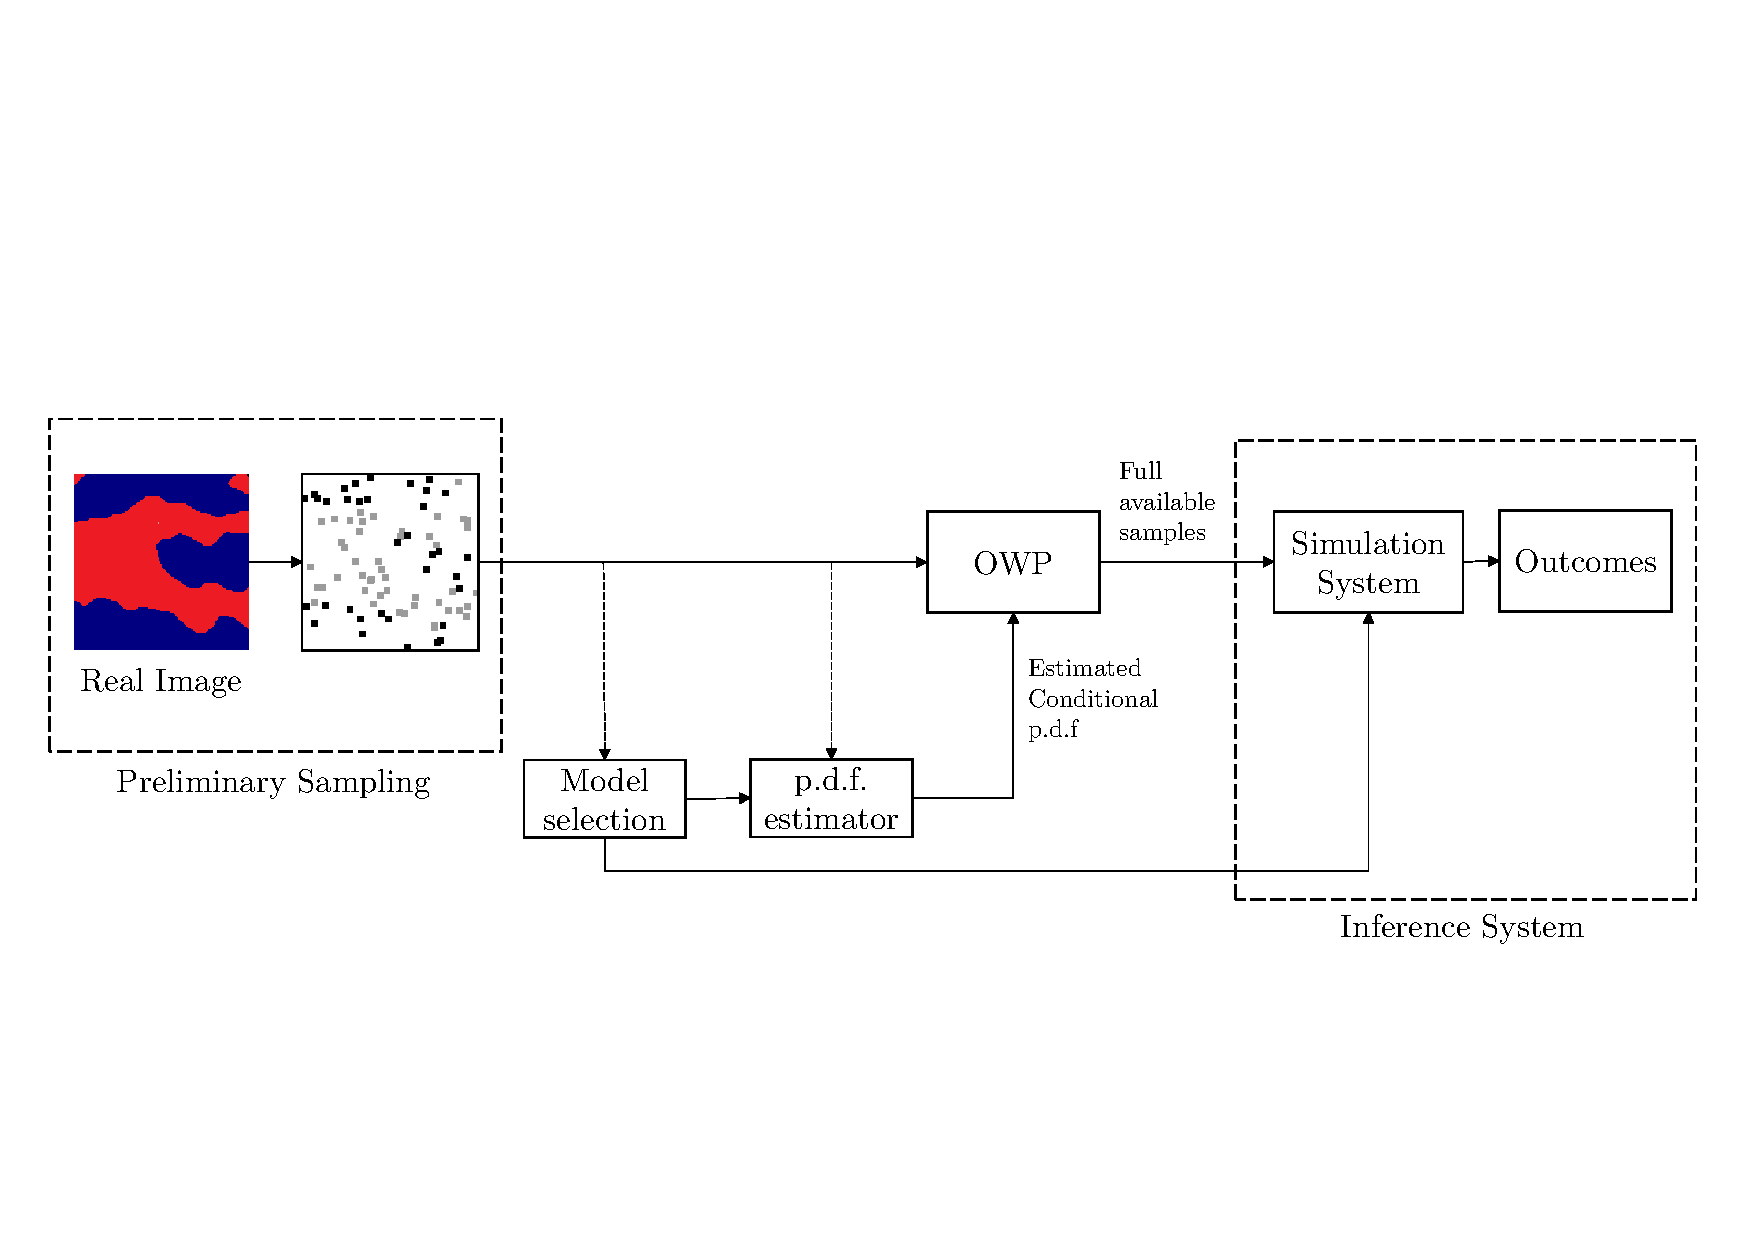
\includegraphics[width=1\columnwidth]{Figures/IDSDAY2015/generic_scheme}
	\caption{\label{fig:gen_scheme} General scheme used}
\end{figure}

The implementation of the different blocks of the proposed system at fig. \ref{fig:gen_scheme} will lead to several practical variants to take advantage of available external information sources. In order to evaluate the \emph{OWP} solutions a  performance comparison with random and structured sampling schemes will be performed.

%We will explore an \emph{OWP} acquisition system where the pixel entropy estimation is based on MPS simulations analysis as presented in fig. \ref{fig:owpmps}.
%
%\begin{figure}[ht!]
    %\centering
    %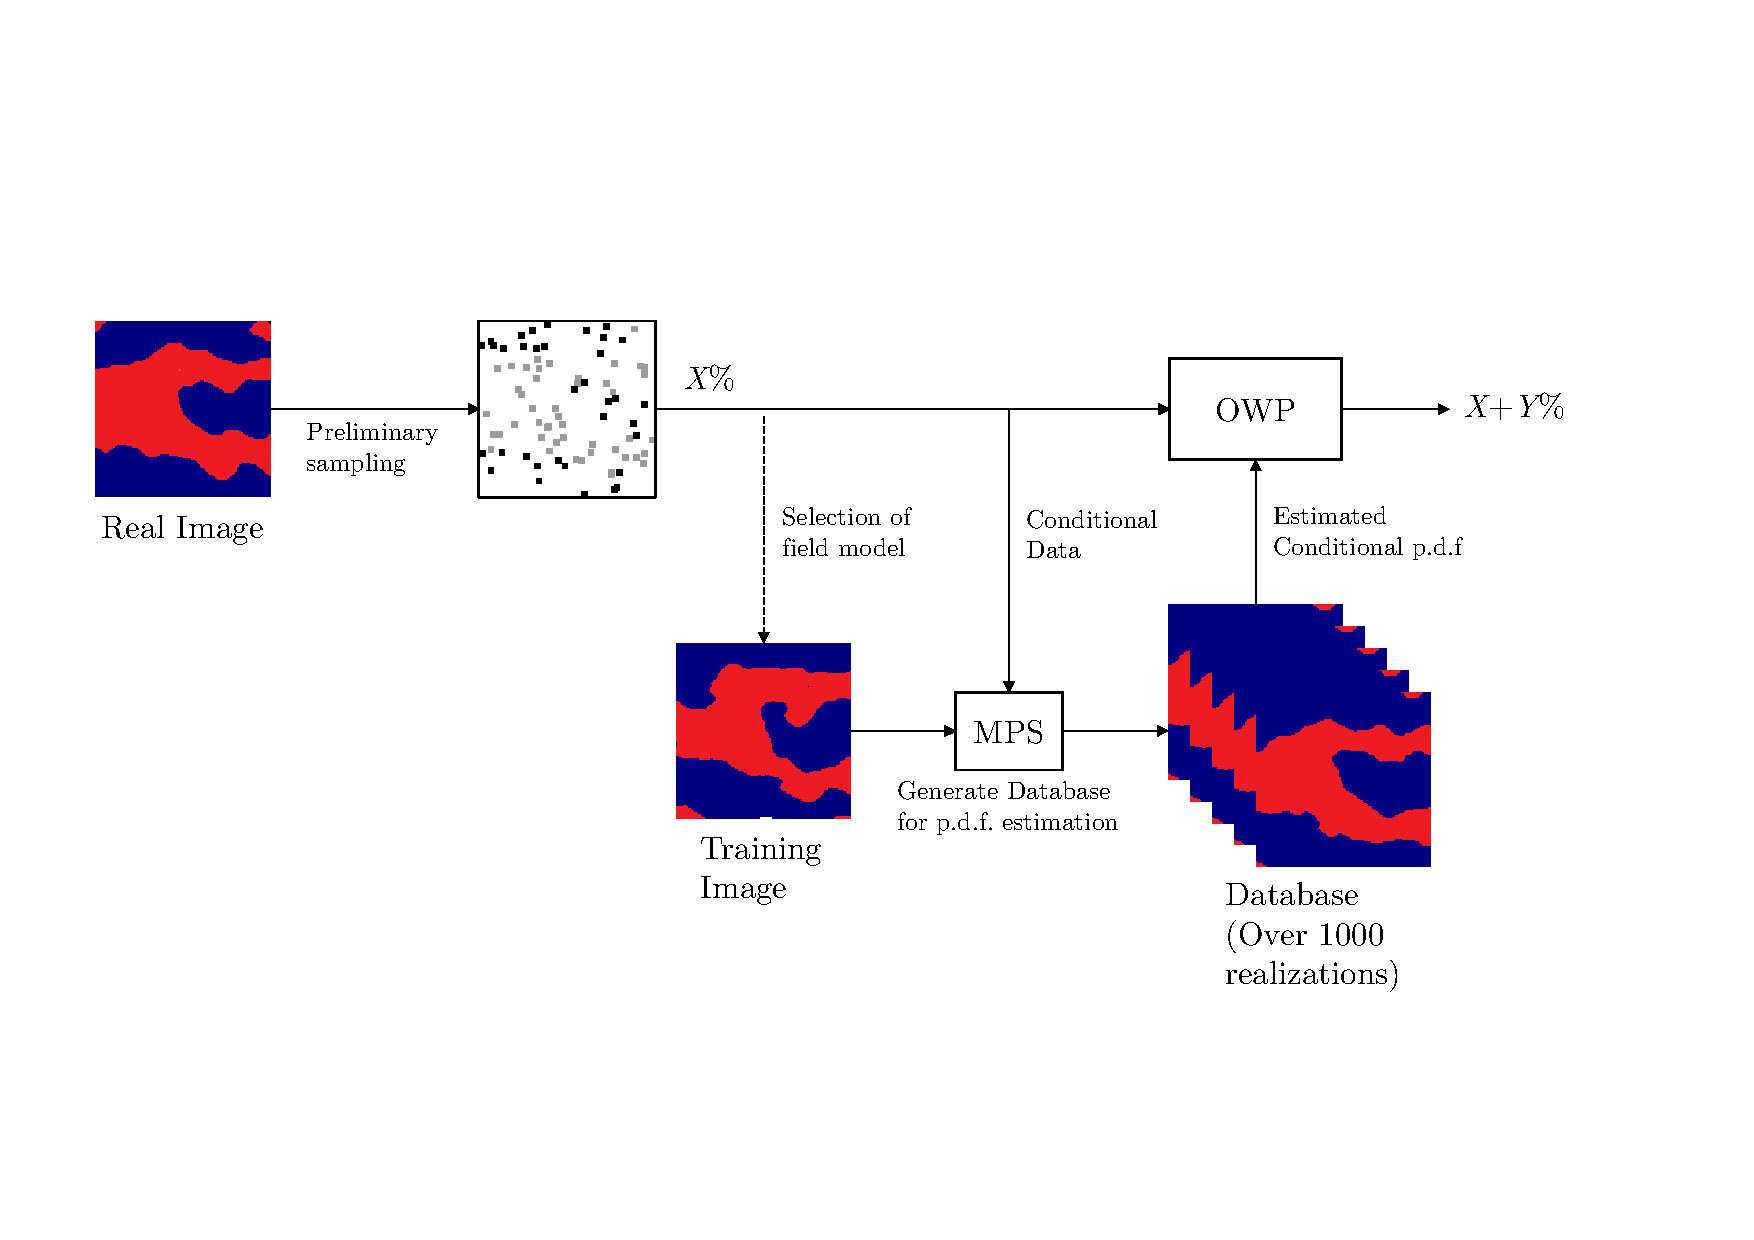
\includegraphics[width=1\columnwidth]{Figures/IDSDAY2015/OWP_MPS}
	%\caption{\label{fig:owpmps} OWP-MPS acquisition scheme}
%\end{figure}
%
%In sequential sensing is possible to update the probabilities after a new observation is available. This MPS enhanced scheme is shown in fig. \ref{fig:owpmpsenhc}.
 %
%\begin{figure}[ht!]
    %\centering
    %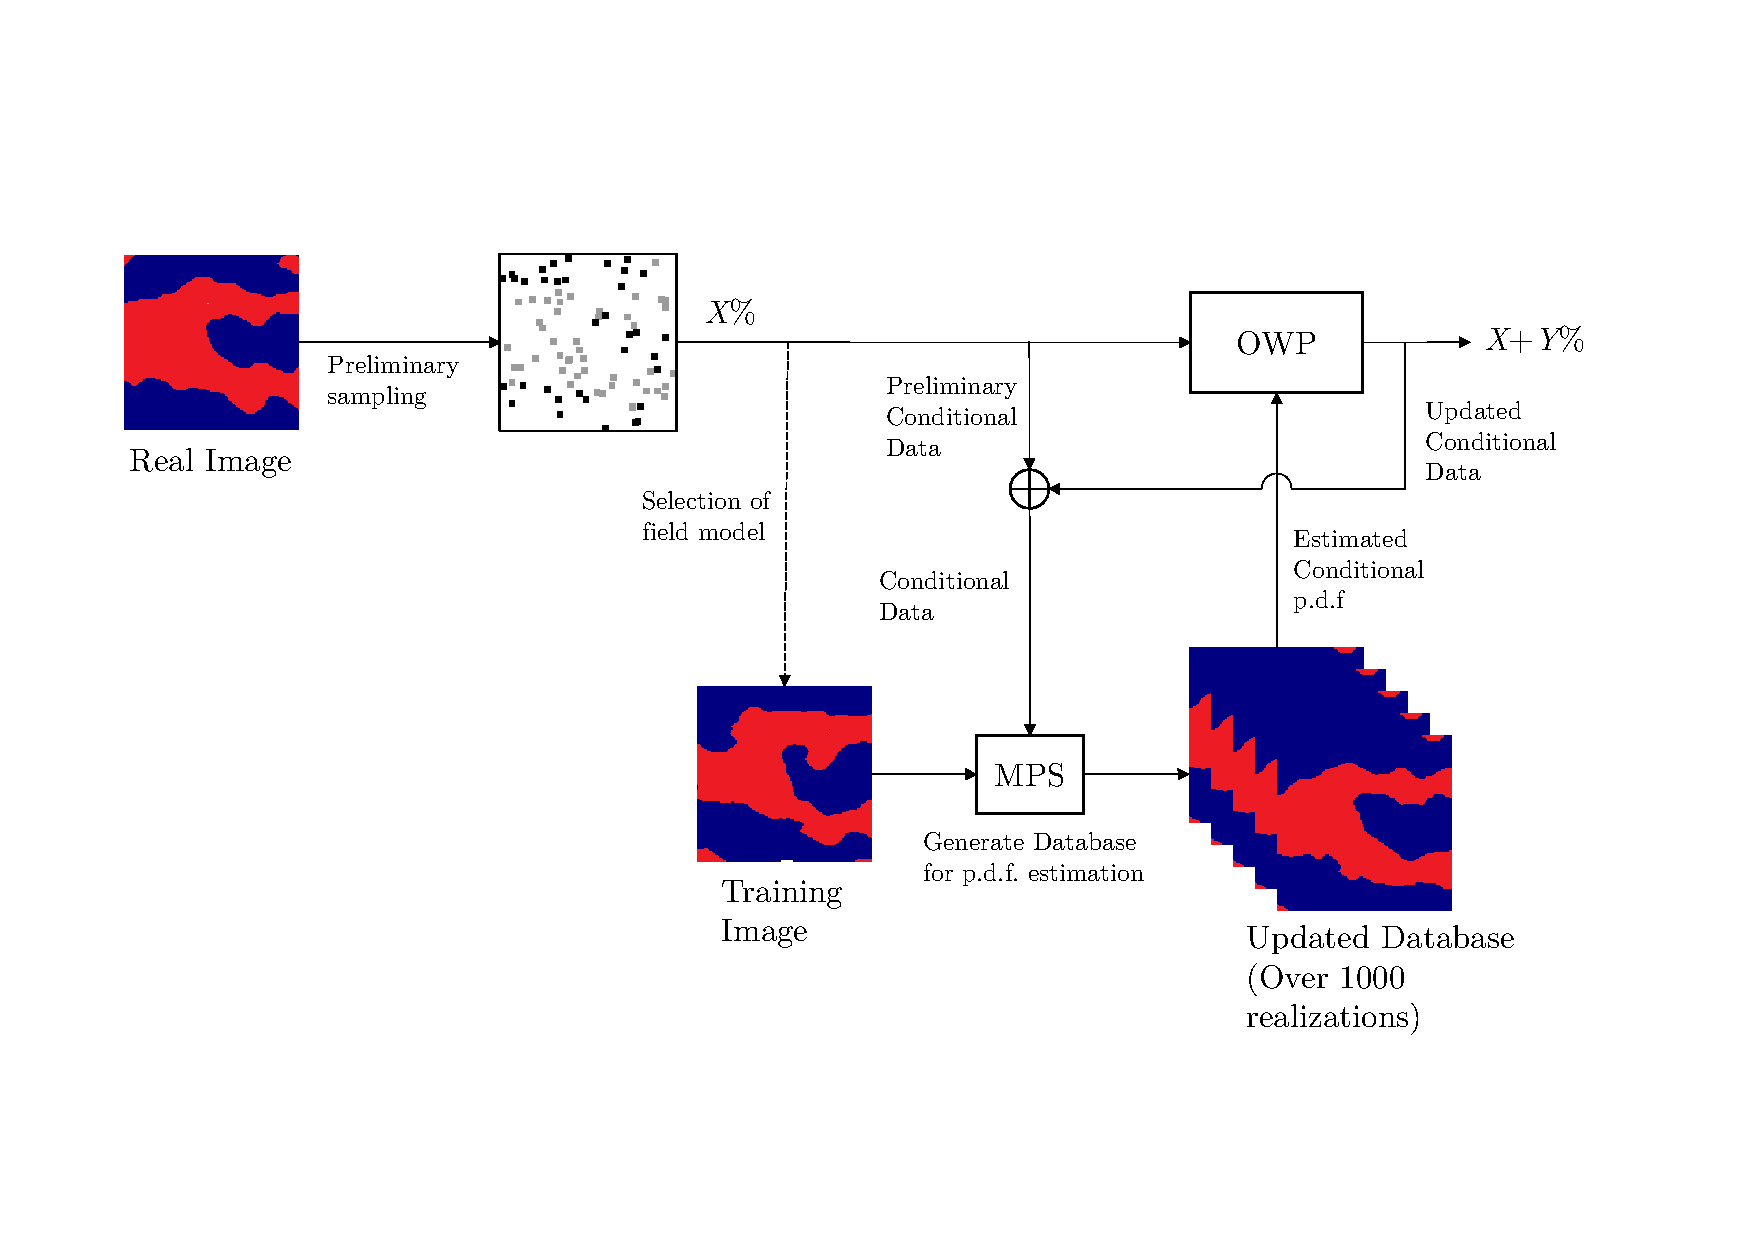
\includegraphics[width=1\columnwidth]{Figures/IDSDAY2015/OWP_MPS_ENHACED}
	%\caption{\label{fig:owpmpsenhc}OWP-MPS Enhanced acquisition scheme}
%\end{figure}
%
%Finally, we propose to bypass the use of \emph{MPS} and use the training image instead by pattern search based probabilities estimation (fig. \ref{fig:owptips}).
%
%\begin{figure}[ht!]
    %\centering
    %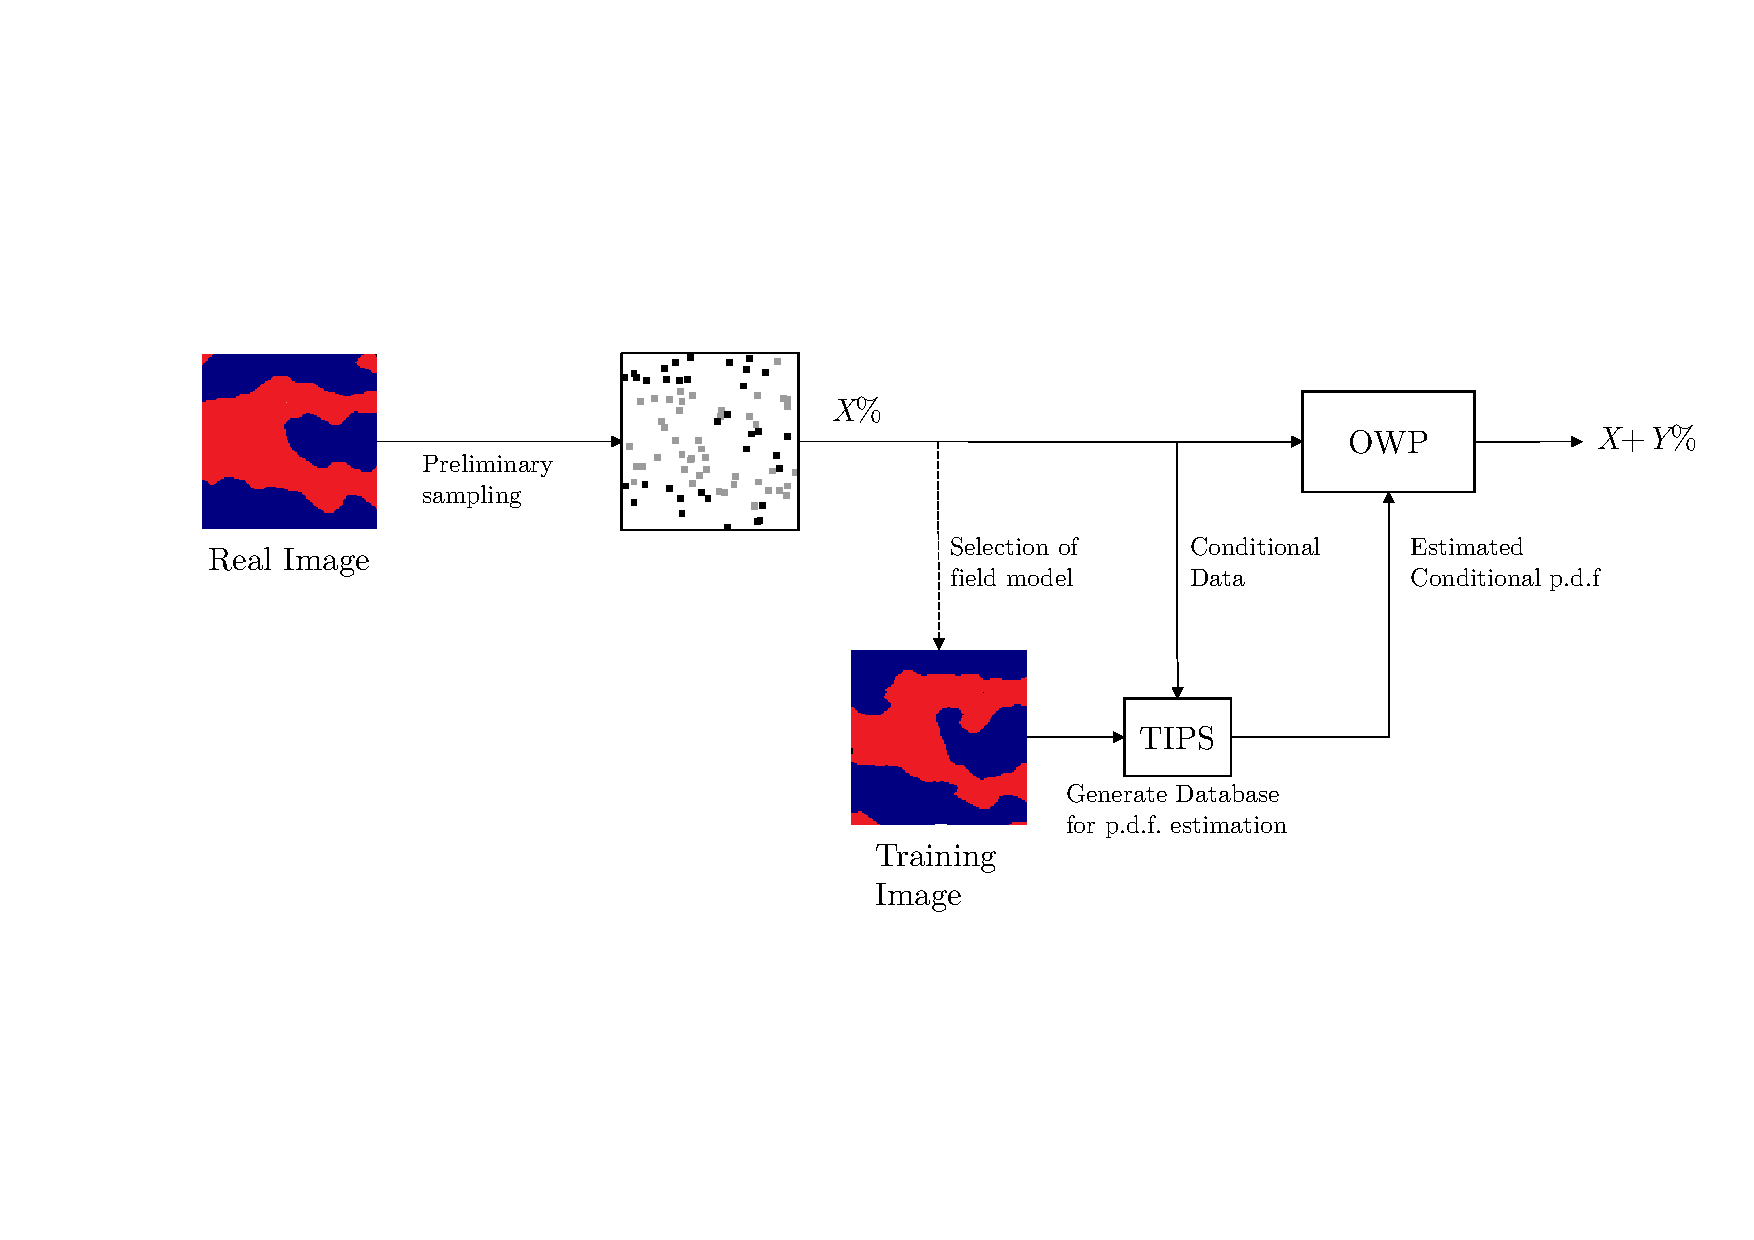
\includegraphics[width=1\columnwidth]{Figures/IDSDAY2015/OWP_TIPS}
	%\caption{\label{fig:owptips} TIPS acquisition scheme}
%\end{figure}
%






























































































































	
	
%\section{Time measurement}

%All implementation and testing tasks will be executed at a $6$ cores processor CPU Intel(R) Xeon(R) $E5-2630$ $v2$ with $2.60$ Ghz, and $16.0$ GB of ram at $1866$ MHz, working under Windows $10$ operative system and Matlab $8$ ($R2014a$). Comparison between proposed approaches will be performed in order to evaluate the improvement achieved for the selected database and the computational demand required for each approach.


\section{Performance Metrics}

The performance metrics consider both field reconstruction quality analysis and variability of conditioned simulations.

For reconstruction, comparisons between the original image and the reconstructions will be performed. Classical indicators assess the quality of a \emph{2-D} image, $X$, by comparing it with a reference \emph{2-D} image, $Xr$, \cite{Gonzalez2002_a} with both images of size $M_u$ by $M_v$.

The signal to noise ratio \emph{SNR} expressed in decibels \emph{dB}:

\begin{equation}
\label{eq:ImQuality_SNR}
	\mathbf{SNR} = 10 \cdot log_{10} \left( \frac{\sum_{u = 1}^{M_u}{ \sum_{v = 1}^{M_v}{ \left| Xr_{u,v} \right|^2 } }}{\sum_{u = 1}^{M_u}{ \sum_{v = 1}^{M_v}{ \left| Xr_{u,v} - X_{u,v} \right|^2 } }} \right)
\end{equation}

The peak signal to noise ratio \emph{PSNR} expressed in decibels \emph{dB}:

\begin{equation}
\label{eq:ImQuality_PSNR}
	\mathbf{PSNR} = 10 \cdot log_{10} \left( \frac{ max( Xr_{u,v} )^2 }{\frac{1}{M_u \cdot M_v} \cdot \sum_{u = 1}^{M_u}{ \sum_{v = 1}^{M_v}{ \left| Xr_{u,v} - X_{u,v} \right|^2 } }} \right)
\end{equation}


The root mean square error \emph{RMSE}:

\begin{equation}
\label{eq:ImQuality_RMSE}
	\mathbf{RMSE} = \sqrt{\frac{1}{M_u \cdot M_v} \cdot \sum_{u = 1}^{M_u}{ \sum_{v = 1}^{M_v}{ \left| Xr_{u,v} - X_{u,v} \right|^2 } }}
\end{equation}

The mean absolute error \emph{MAE}:

\begin{equation}
\label{eq:ImQuality_MAE}
	\mathbf{MAE} = \frac{1}{M_u \cdot M_v} \cdot \sum_{u = 1}^{M_u}{ \sum_{v = 1}^{M_v}{ \left| Xr_{u,v} - X_{u,v} \right| } }
\end{equation}

On the other hand, the structural similarity index \emph{SSIM} tries to estimate the similarity between two images by emulating the human perception \cite{Wang_2004_a}. A simplified version of this indicator is given by:

\begin{equation}
\label{eq:ImQuality_SSIM}
	\mathbf{SSIM}(X,Xr) = {(2\mu_{X} \mu_{Xr} +c_{1})(2{\sigma}_{X, {Xr}}+c_{2})\over ({\mu_X}^{2}+{\mu}_{Xr}^2+c_{1})({\sigma}_{X}^{2}+{\sigma}_{Xr}^{2}+c_{2})}
\end{equation}

Here, $\mu_{X}$ ($\mu_{Xr}$) and $\sigma_{X}$ ($\sigma_{Xr}$) denote the average and variance of $X$ ($Xr$), respectively. $\sigma_{X, Xr}$ is the covariance of $X$ and $Xr$. $c_{1}$ and $c_{2}$ are required to stabilize the division.

For our problems, outcomes are the sensing locations provided for each method. Then, we don’t have any reconstruction in order to compare different approaches. Thus, an alternative quality analysis based on the variability of simulations conditioned by the obtained sensing locations is proposed. Then, we can estimate the mean and standard deviations from simulations for each implemented well placement approach.

Another analysis is to evaluate the global behavior of simulations in relation with the target field. We propose the $SNR$ indicator between the mean of simulations and the reference image and the mean of the $SNR$ of each simulation and the reference image. Finally we propose to use some reconstruction method from data measured at sensing locations like total variation inpainting.


